\documentclass{article}
\usepackage[left=0.85in,top=0.6in,right=0.85in]{geometry}
\usepackage{booktabs}
\usepackage{array,multirow}
\usepackage{graphicx}
\usepackage{pifont}
\usepackage{amssymb}
\usepackage{enumitem}
\usepackage{floatflt}
\usepackage{hyperref}
\usepackage[table]{xcolor}

\title{\Huge Cherry Dropper}
\author{\huge Group 26}
\begin{document}
\maketitle
\begin{center}
\setlength{\arrayrulewidth}{1mm}
\setlength{\tabcolsep}{18pt}
\renewcommand{\arraystretch}{2.5}
 
{\rowcolors{3}{green!80!yellow!50}{green!70!yellow!40}
\begin{tabular}{ |p{3cm}|p{3cm}|  }
\hline
\multicolumn{2}{|c|}{\huge Optimus} \\
\hline
 ROLL NO.  & NAME\\
\hline
 140050029 & B.Avinash \\
 140050069   & Suraj Geddam \\
 140050087 & Ashna Gaur \\
\hline
\end{tabular}
}
\\[5\baselineskip]
{\huge CS251 Project- Box 2D}
\\[2\baselineskip]
Prepared for Software Systems lab: \\[1\baselineskip]
{\large Instructor} : \textbf{Prof. Sharat Chandran }\\[1\baselineskip]
Autumn 2015 \\
\end{center}

\newpage
\section*{\huge Table of Contents:} \label{Contents}
\begin{enumerate}
    \LARGE  \item Introduction
    \begin{enumerate} [label*=\arabic*.]
        \large \item Project Design
        \large \item Description
    \end{enumerate}
    \LARGE  \item Objects of the Project
    \begin{enumerate} [label*=\arabic*.]
        \large \item Pendulum
        \large \item Dominos
        \large \item Gears
        \large \item Train of small spheres
        \large \item Hydraulic lift
        \large \item Revolving plank
        \large \item Another Dominos
        \large \item Fluid in the box
        \large \item The boat 
        \large \item Pulley joint
        \large \item Cake 
    \end{enumerate}
    \LARGE  \item Software Applications Implemented
    \begin{enumerate} [label*=\arabic*.]
        \large \item Documentation
        \large \item Profiling
        \large \item Webpage Preparation
        \large \item Makefiles
    \end{enumerate}
    \LARGE  \item Methods
    \begin{enumerate} [label*=\arabic*.]
        \large \item Box2D Engine
        \large \item Git
        \large \item Makefile
        \large \item Gprof
        \large \item Doxygen
        \large \item HTML, CSS
        \large \item Latex
    \end{enumerate}
    \LARGE  \item Work Distribution
    \begin{enumerate} [label*=\arabic*.]
        \large \item B.Avinash
        \large \item Suraj Geddam
        \large \item Ashna Gaur
        \large \item Honour Code
    \end{enumerate}
    \LARGE  \item Difficulties and Deviations
    \begin{enumerate} [label*=\arabic*.]
        \large \item Difficulties Faced And how we overcame them
        \large \item What we didn't implement
    \end{enumerate}
\end{enumerate}
\clearpage
 
\begin{figure}[h]
\centering
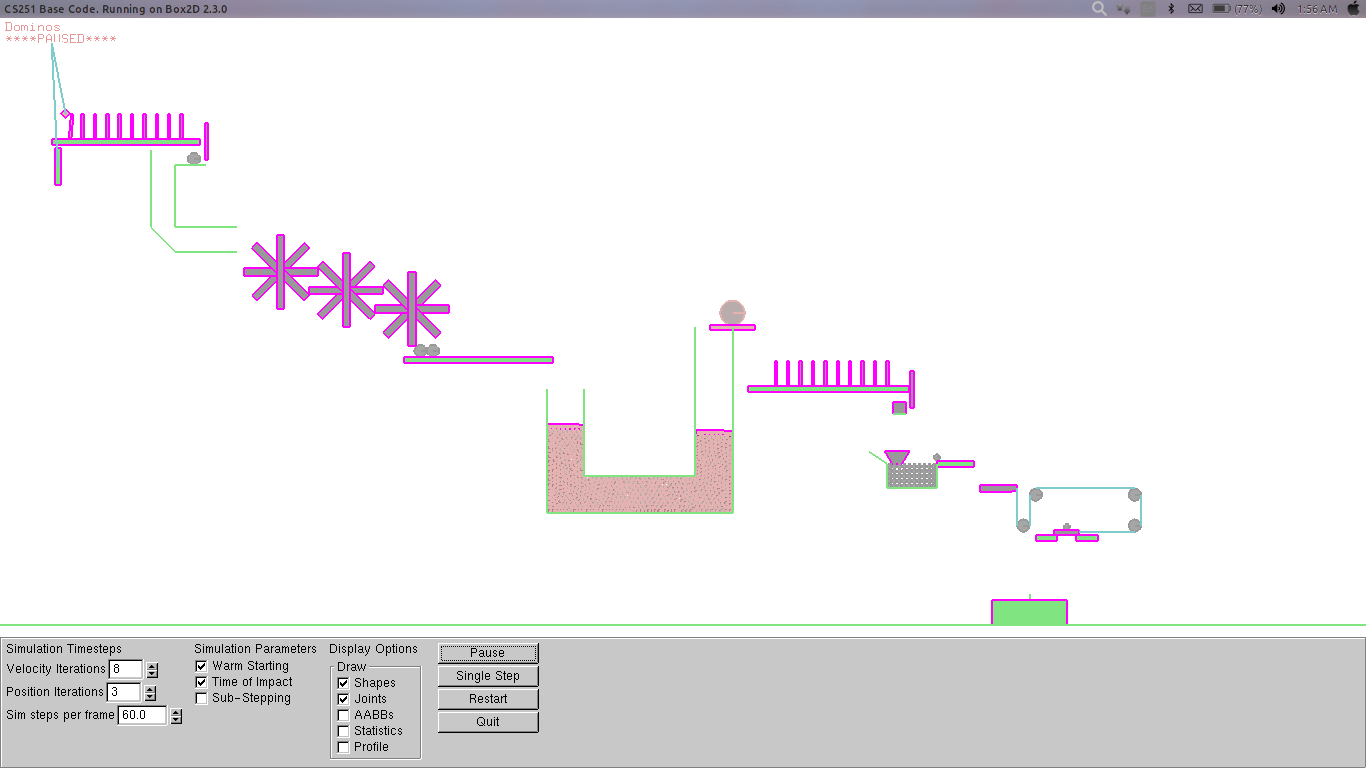
\includegraphics[width=1 \linewidth]{suraj.png}
\caption{\large Our Box2D Design}
\end{figure}
\begin{itemize}
	\item[] \textbf{\LARGE Project Design} \vspace{0cm} \\
	\large This project idea is a simulation which is based on placing a cherry on the cake.We were inspired from many daily-life simulations and by the one given in the Lab03 .  \vspace{0.4cm}
	\item[] \textbf{\LARGE Description} \vspace{0cm} \\
	\large In this simulation, the bob of the left most pendulum hits the first domino which in return hit one by one and finally the revolving domino hits the small ball which goes and turns the 3 gears and in turn initiates a train of small balls to go and fall on a hydraulic lift  which makes the heavy ball on the plank on the right top of the lift. The heavy ball initiates the dominos to go and hit the small box.\\
 \end{itemize}
\clearpage

\begin{itemize}
 \item[] \textbf{\LARGE Objects of the Project} \\
        \begin{itemize}[label=$\blacksquare$] \vspace{0cm}
            \item \textbf{\Large Pendulum} 
        \end{itemize}
        \large Pendulum at the top left corner in the below image is the start of the simulation. The bob hits the first domino. \\ \vspace{0.55 cm}

        \begin{itemize}[label=$\blacksquare$] \vspace{0cm}
            \item \textbf{\Large Dominos } 
        \end{itemize} 
        \large The first domino which in return hit one by one and finally the revolving domino hits the small ball which goes to the gears. \\ \vspace{0.55 cm}

        \begin{itemize}[label=$\blacksquare$] \vspace{0cm}
            \item \textbf{\Large Gears } 
        \end{itemize}
        \large The small ball rotates the first gear anti-clockwise which rotates the second gear in clockwise and thus the third gear rotates in anti-clockwise direction and hits the train of small spheres .\\ \vspace{0.55 cm}

        \begin{itemize}[label=$\blacksquare$] \vspace{0cm}
            \item \textbf{\Large Train of small spheres } 
        \end{itemize}
        \large The train of these spheres follow the same as the dominos above and fall on one side of the Hydraulic lift.\\ \vspace{0.65 cm}
        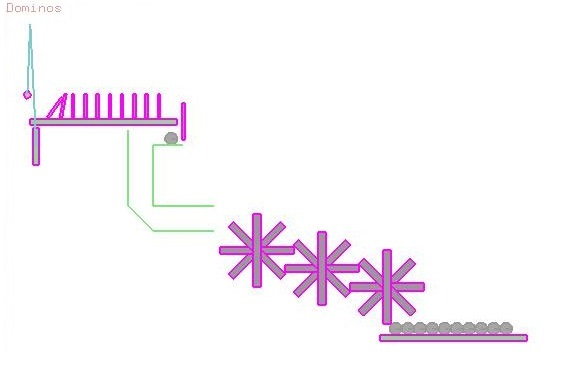
\includegraphics[width=1 \linewidth]{avinash.jpg}\\

        \begin{itemize}[label=$\blacksquare$] \vspace{0cm}
            \item \textbf{\Large Hydraulic lift } 
        \end{itemize}
        \large The name itself indicates the function.The balls on one side of the lift cause the rise of height to the other side due to which the plank hits the revolving plank. \\ \vspace{0.65 cm}

        \begin{itemize}[label=$\blacksquare$] \vspace{0cm}
            \item \textbf{\Large Revolving plank } 
        \end{itemize}
        \large The revolving plank is set on the right most end of the Hydraulic lift and a heavy sphere is placed on the plank.\\ \vspace{0.65 cm}

        \begin{itemize}[label=$\blacksquare$] \vspace{0cm}
            \item \textbf{\Large Another Dominos } 
        \end{itemize}
        \large The heavy sphere on the plank falls on the dominos and intiates them to hit the small box placed to the left of revolving domino.\\ \vspace{0.65 cm}
        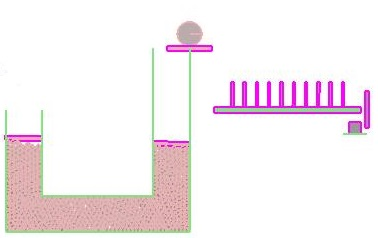
\includegraphics[width=1 \linewidth]{ashna.jpg}\\
\clearpage

        \begin{itemize}[label=$\blacksquare$] \vspace{0cm}
            \item \textbf{\Large Fluid in the box } 
        \end{itemize}
        \large You may see the doxygen generated documentation in the doc directory after running make codeDoc in the terminal. Documentation of code is a necessity for other programmers to understand our code.\\ \vspace{0.65 cm}

        \begin{itemize}[label=$\blacksquare$] \vspace{0cm}
            \item \textbf{\Large the boat} 
        \end{itemize}
        \large Our code profile can be generated by running make profile. It will be available in doc directory. We used it to see where the code is consuming the most time and needs optimisation. \\ \vspace{0.65 cm}

        \begin{itemize}[label=$\blacksquare$] \vspace{0cm}
            \item \textbf{\Large Pulley Joint} 
        \end{itemize}
        \large We made a webpage and a presentation of our Brick Breaker game. You can go to the webpage at \url{www.cse.iitb.ac.in/~shrey}\\ \vspace{0.65 cm}
        
        \begin{itemize}[label=$\blacksquare$] \vspace{0cm}
            \item \textbf{\Large Cake} 
        \end{itemize}
        \large Makefile is what brings it all together. We used makefile to compile multiple files, generate documentatioon, do code profiling and remove waste files.\\ \vspace{0.65 cm}
	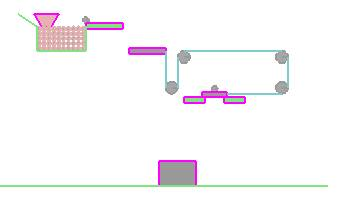
\includegraphics[width=1 \linewidth]{suraj.jpg}\\
    \end{itemize}

\begin{itemize}
	\item[] \textbf{\LARGE Software Applications Implemented} \\
        \begin{itemize}[label=$\blacksquare$] \vspace{0cm}

            \item \textbf{\Large Documentation }\\
            \large We used doxygen to document our project.We have written meaningful comments in order to increase the understandability of other programmers who try to understand our project. We can get the documentation by writing "make doc" in the project direcory(on the terminal). \vspace{0.60 cm}

            \item \textbf{\Large Profiling}\\ 
            \large The code profile can be generated by the command "make profile" in the project directory . \vspace{0.60 cm}

            \item \textbf{\Large Webpage Preparation}\\ 
            \large We created a webpage for the project which is available at {\large {\bf HOMEPAGE:} \ \url{www.cse.iitb.ac.in/~avinash}}. \vspace{0.60 cm}

            \item \textbf{\Large Makefile}\\ 
            \large We created a makefile which can be used to cmpile all the files, do the profiling, create the executables, create the documentation of the project ,report of the project and clean all the unneccessary files. \vspace{0.60 cm}


 \end{itemize}
        \end{itemize}
    \clearpage

\begin{itemize}
	\item[] \textbf{\LARGE Methods} \\
        \begin{itemize}[label=$\blacksquare$] \vspace{0cm}

            \item \textbf{\Large Box2D Engine }\\
            \large Box2D is an open source C++ engine for simulating rigid bodies in 2D.We learnt about the Box2D engine in our lab03. We created bodies, fixtures, shape and set their physical properties like friction, restitution, colour \cite{colour}.\vspace{0.60 cm}

            \item \textbf{\Large Makefile }\\ 
            \large Using makefiles \cite{Makefile} was an important technique we learned in the lab. Makefile shortens our work by compiling all the required files, profiling them,creating executables and cleaning the unneccessary stuff. \vspace{0.60 cm}

            \item \textbf{\Large Git }\\ 
            \large Git is a widely used version control system for software development. It is a distributed revision control system with an emphasis on speed, data integrity, and support for distributed, non-linear workflows .Git \cite{Git} is one of the most important technique a software engineer must know. We learned to keep version control of our project in Lab07. Git stores all vesions of the project we push into it and is very useful when we want the previous version of the code. \vspace{0.60 cm}

            \item \textbf{\Large Doxygen }\\ 
            \large Doxygen is the de facto standard tool for generating documentation from annotated C++ sources, but it also supports other popular programming languages such as C, Objective-C, C++, PHP, Java, Python, IDL (Corba, Microsoft, and UNO/OpenOffice flavors), Fortran, VHDL, Tcl, and to some extent D. This makes easier for others to understand a code. We used Doxygen \cite{Doxygen} to generate the documentation in HTML which we learnt in Lab09.  \vspace{0.60 cm}

            \item \textbf{\Large Gprof }\\
            \large Gprof is a profiling program which collects and arranges statistics on your programs.Basically, it looks into each of your functions and inserts code at the head and tail of each one to collect timing information. We optimised our code using gprof as much as we could which we learnt in our Lab09 . \vspace{0.60 cm}

            \item \textbf{\Large HTML, CSS }\\
            \large We created a web page for the box2d project maded by us using basic HTML and CSS knowledge which we learnt in our Lab02.\vspace{0.60 cm}

            \item \textbf{\Large Latex }\\ 
            \large LaTeX is a high-quality typesetting system; it includes features designed for the production of technical and scientific documentation. LaTeX is the de facto standard for the communication and publication of scientific documents. We made our project report and the presentation in latex which we learnt in our Lab06. \vspace{0.60 cm}
 \end{itemize}
        \end{itemize}
    \clearpage

\begin{itemize}
	\item[] \textbf{\LARGE Work Distribution} \\
	   \begin{itemize}[label=$\blacksquare$] \vspace{0cm}
           \item \textbf{\Large B.Avinash }\\
           \large Roll Number: 140050029\\ Contribution: 100\% \\ The project was divided into 3 parts which was assigned to the 3 members of the group. Avinash did the first part i.e, the part involving gears and documented his part. He also prepared the report for the project and made the profiling. \vspace{0.65 cm}
           \item \textbf{\Large Suraj Geddam }\\ 
           \large Roll Number: 140050069\\ Contribution: 100\% \\ Suraj did the third and final part of the project which invloves the fluid part and documented his part. He also created the makefile.\vspace{0.65 cm}
           \item \textbf{\Large Ashna Gaur }\\ 
           \large Roll Number: 140050087\\ Contribution: 100\% \\  Ashna did the second part of the project which involved hydraulic lift and documented her completely. She also created the project webpage. \vspace{0.65 cm}
       \end{itemize}
       \item[] \textbf{\LARGE Honour Code} \\ 
       \large We pledge on our honour that we have not given or received any unauthorized assistance on this assignment or any previous task.\\\vspace{0.4 cm}
    \clearpage   

	\item[] \textbf{\LARGE Difficulties and Deviations} \\
	\item[] \textbf{\Large Difficulties Faced And how we overcame them} \\
    \large The parts where we faced the main difficulties were to create gears , hydraulic lift and fluid. We tried to understand the code in the gers.h file present in testbed and completed the gears part. And we used small balls in the hydraulic lift instead of fluid which worked fine for us and even looked good.\\ \vspace{0.4 cm}

    \item[] \textbf{\Large What we didn't implement} \\ 
Our intial design was the picture below.
\begin{figure}[h]
\centering
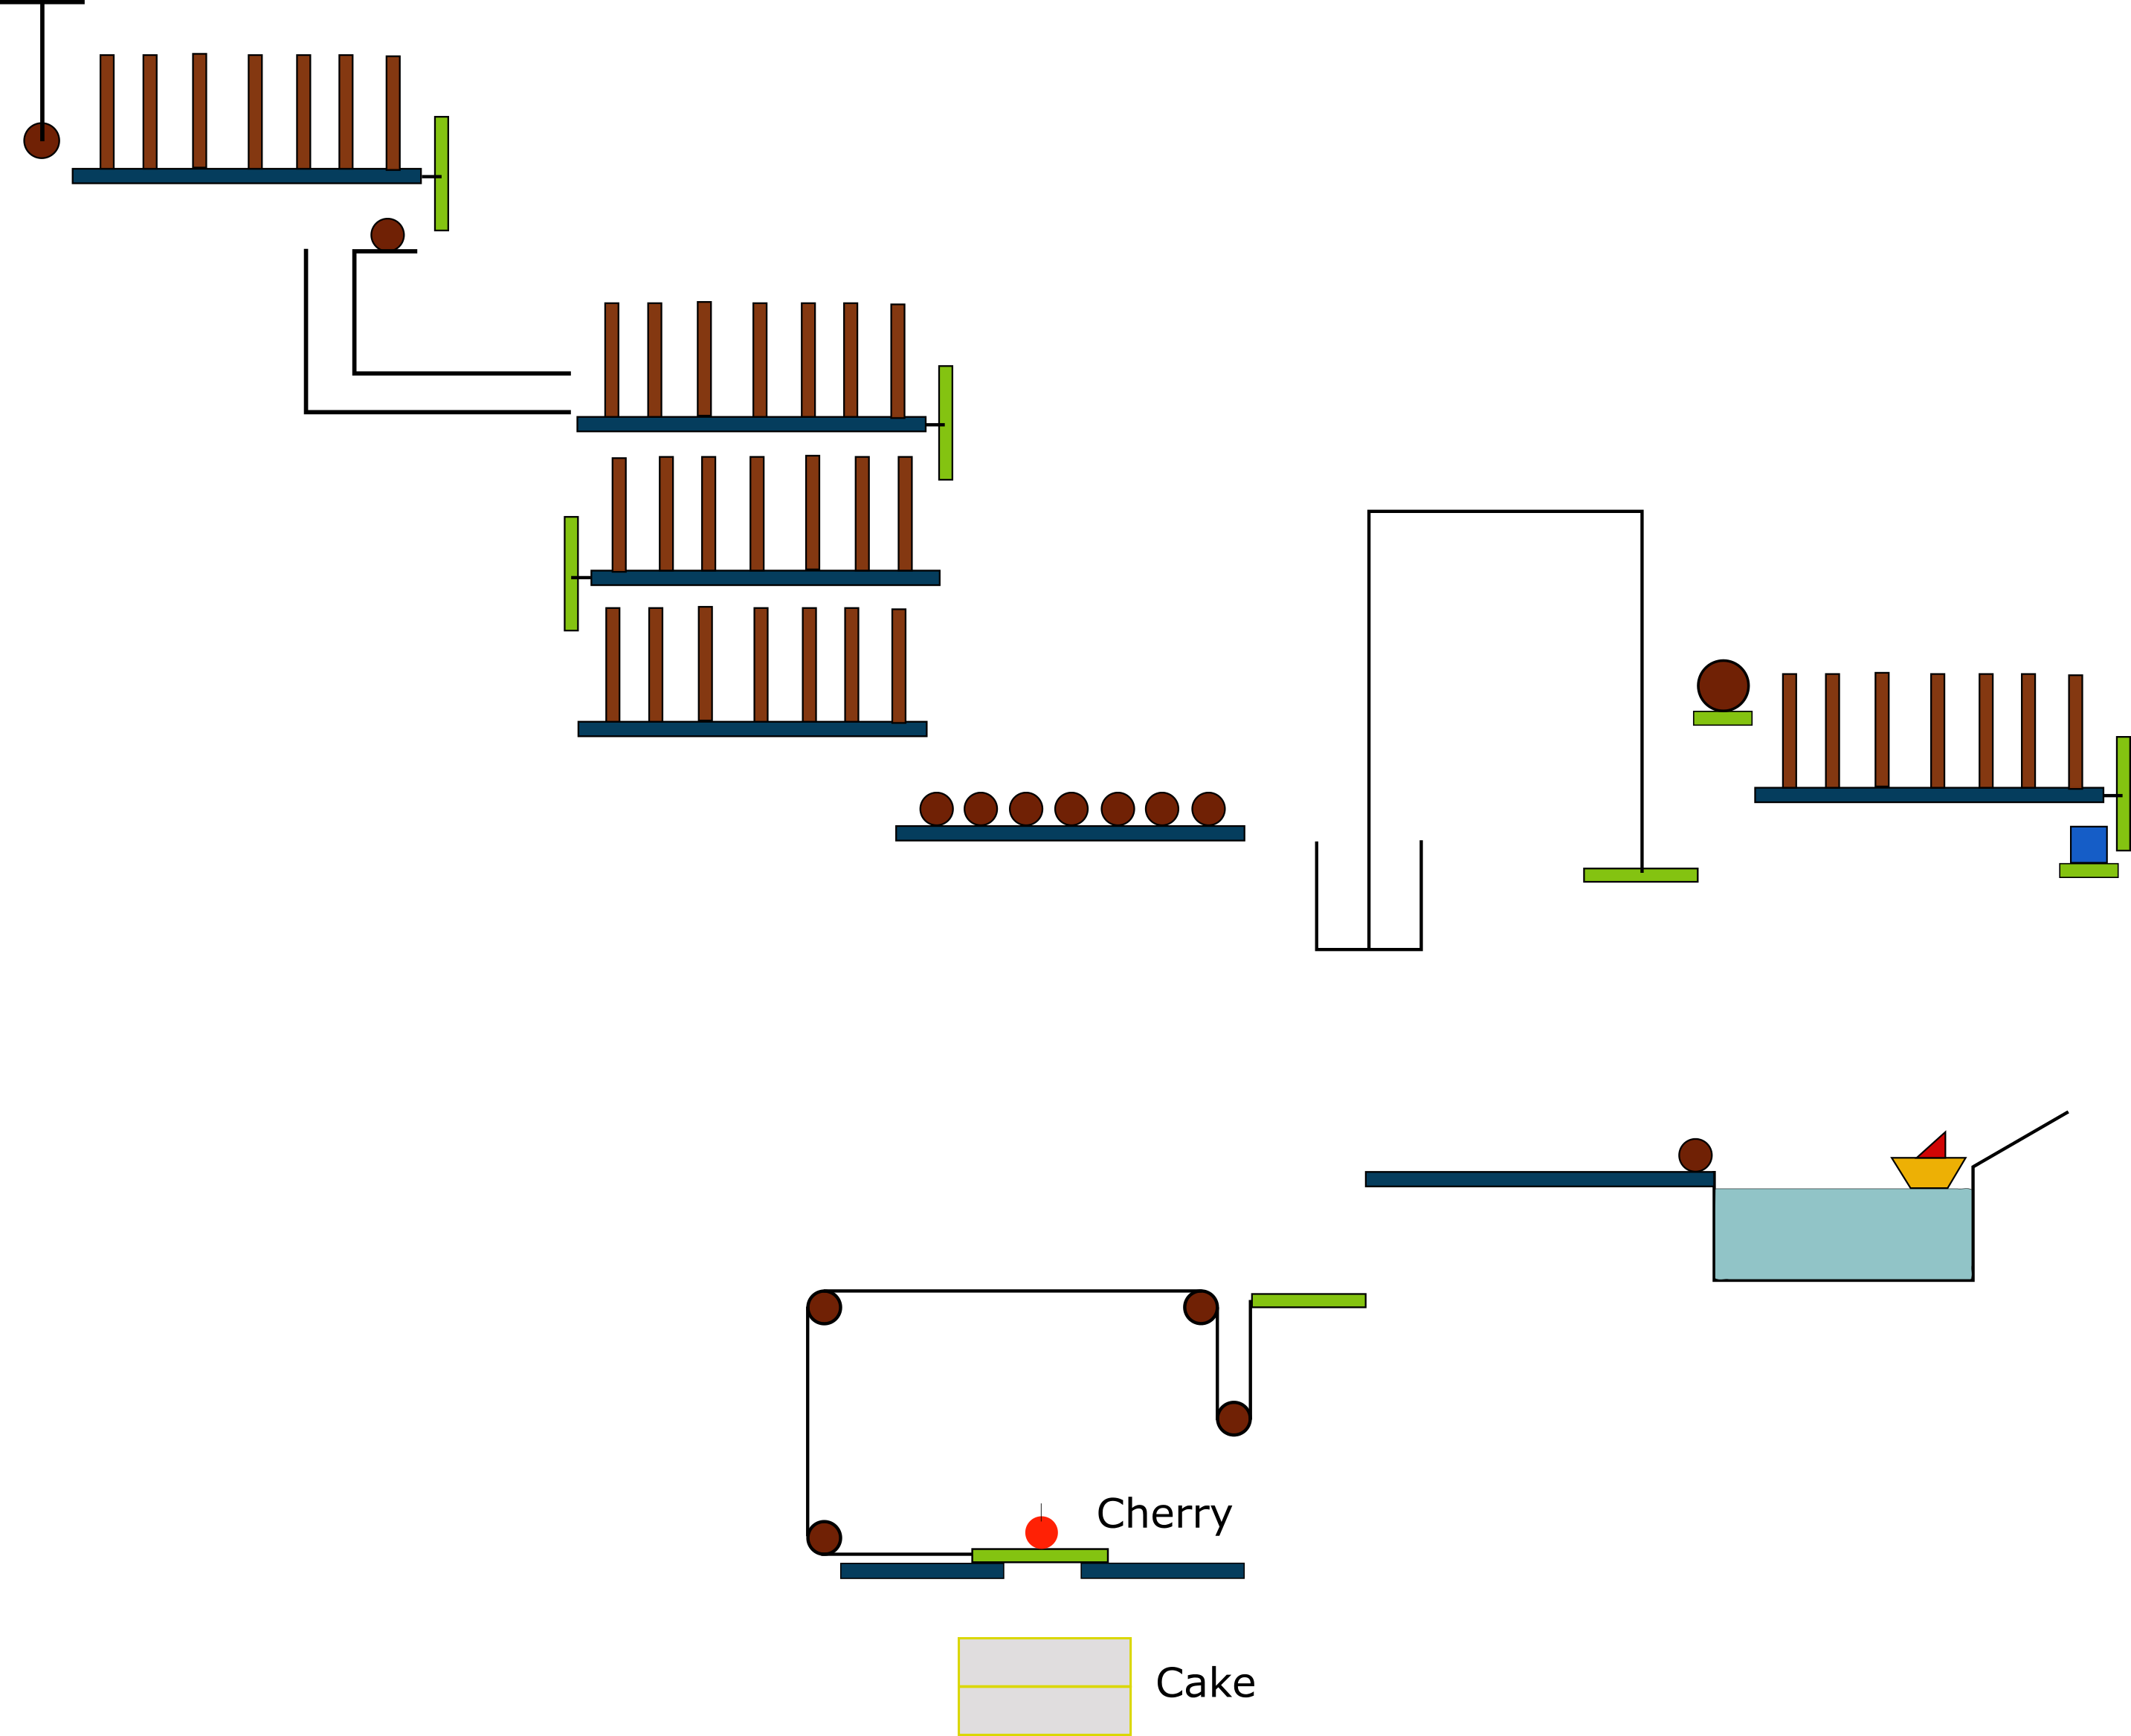
\includegraphics[width=1 \linewidth]{box2D.png}
\caption{\large Our Box2D Design}
\end{figure}
But the TA gave us the suggestion to implement gears and simulation of gaseos particles to make it a bit cool. Because this design was pretty similar to the base code and was looking pretty easy. So, we increased the complexity in the design to achieve what we did now.
\\ \vspace{0.4 cm}

\end{itemize}

\bibliography{report}
\bibliographystyle{plain}
\end{document}

